\chapter{Multicore DSP in Video Stream Processing}
\label{chapter:experiments}
The objective of this thesis is to understand the performance of the Texas Instruments implementation of Open Event Machine in stream processing. The objective is achieved by implementing a video stream processing application using OpenEM, measuring its performance and comparing that to a comparable, statically scheduled application. The comparable application is implemented using the PREESM framework. Both of the applications are instrumented in similar manner.

In this chapter the material and methods used in the experiment are introduced. The performance and behavior of OpenEM is evaluated using quantitative analysis. The analysis methods are explained in section \ref{sec:performance-analysis}. The hardware platform used in the experiments is the Texas Instruments TMS320C6678, which is described in \ref{sec:c6678}. PREESM provides the tools for implementing the comparable workload. PREESM is introduced in section \ref{sec:preesm}. The workload application processes video streams. An overview to video streams is provided in section \ref{sec:video-streams}. Finally, the algorithms computed in the stream processing application are part of the Canny edge detection algorithm introduced in \ref{sec:canny}.

\section{Performance Analysis}
\label{sec:performance-analysis}
To understand the behavior and performance of software systems, quantitative data about the system execution is required. Precisely what data is needed depends on the purpose of the analysis. A couple of popular methods for acquiring quantitative data about software systems are introduced in this section. First, an overview to the performance analysis of software systems is provided in the subsection \ref{subsec:analysing-software}. Second, a closer focus to measuring software systems is taken in subsection \ref{subsec:measuring-software}. Finally, the analysis of the acquired data is described in subsection \ref{subsec:data-analysis}.

\subsection{Analysing Software Systems}
\label{subsec:analysing-software}
According to Jain \cite{jain1991art} the performance analysis of software systems can be split into three categories, which are analytical modeling, simulation and measuring of software systems. Analytical modeling and simulation use mathematical models for the analysis of the software systems. Abstract mathematical models of a system can be constructed without access to the system under study. To measure a software system, access to the specific system under study is always required. There are many methods for modeling and simulation of software systems, but in most cases they require less work to implement than the actual system under study. These properties make the analytical modeling and simulation attractive for explorative study of software systems that do not exist yet.~\cite{jain1991art}

The key difference between analytical modeling and simulation is the notion of time present in simulation. Analytical modeling solves the system state at a fixed point in time, in contrast to simulators where the system state is computed iteratively at multiple points in time.~\cite{jain1991art}

Performance analysis is used for many different purposes. For example performance analysis can be used to help choose the best performing hardware platform for certain application, or to explore different configurations of an application. Successful analysis requires careful experiment design. First step to successful performance analysis is method selection. Using simulation or analytical modeling can yield results quickly, but they are not as accurate as measuring the real world system.~\cite{jain1991art}

The execution of a computer program is a complex interaction of hardware and software components and thus the number of parameters of the analysis grows large. Factors are parameters that are varied in the analysis. Factors are selected from among all parameters of the system \cite{jain1991art}. Every factor increases the time it takes to complete the analysis and only few of the parameters are relevant for the result of the analysis. Thus, the factor selection requires clear goals for the analysis and a good understanding of the problem space so that the most relevant factors are chosen. The factor selection of the experiments conducted in this thesis is discussed in section \ref{subsec:parameters-and-factors}.

\subsection{Measuring Software Systems}
\label{subsec:measuring-software}
In this thesis a measurement system consisting of a workload, applications and execution hardware is constructed and its performance is measured. In this subsection a closer look at measuring software systems is taken.

The successful comparison of software systems requires meaningful and reasonably accurate measurements of the systems under study. Measurements are obtained by monitoring the system while it is being subjected to a particular workload \cite{jain1991art}. Often the monitored applications are built for the comparison purpose only and therefore any workload they are subjected to is an approximation of the real world workload that would be processed by their real world application counterparts. These approximate workloads are called synthetic workloads. The use of a synthetic workload gives more control over the test conditions and most importantly makes the experiments repeatable.~\cite{jain1991art}

Synthetic workload creation requires care because it needs to mimic its real world counterpart with high accuracy to provide useful any information. Performance analysis is often conducted to understand the performance or feasibility of a software component or a system that does not exist yet. In such situations synthetic workloads need to be used out of necessity.  

The workload is the target of the measurements but it does not define the exact measurements that are to be conducted. Selection of metrics is equally important as the selection of the workload for successful analysis. The best metrics for a given analysis are determined by what is the goal of the analysis. \cite{jain1991art} For example measurements can be used for comparison of throughput of two comparable software systems. In that case clearly a good measure of throughput is needed.

The software measurement tools are called monitors, which can be implemented both in hardware and in software. Monitors are classified to software monitors, hardware monitors, firmware monitors or hybrid monitors depending on the implementation level of the monitor. The implementation level of the monitor affects the level of events that are convenient to measure with it. For example hardware monitors can monitor the state of registers and hardware counters but have difficulties in observing the status of software constructs such as the execution of functions. The software monitors on the other hand can be used to monitor the status of software components but gathering information about the status of the hardware is more difficult and in some cases impossible. \cite{jain1991art} For example it is very complicated to determine whether a memory operation hit a given level of cache or not using software alone but many hardware platforms offer hardware counters to monitor the cache hits and misses.

\subsection{Analysis of the Measurement Data}
\label{subsec:data-analysis}
The goal of the performance analysis is to get actionable results about the systems under study. The data obtained from the models or measurements is not in itself enough for making well-grounded decisions. The models and measurements may yield millions of values for the observed variables and the analyst needs to decide how to best represent the data so that the phenomena behind the data are explained \cite{jain1991art}.

Statistical methods are used to analyze the numerical data and expose the causation and correlation between the factors and the results. Often in the literature simple statistical tools such as mean, mode and standard deviation are used to represent the data in only a few numbers. Such simple statistics are enough if they capture the relevant information about behavior of the system. For example if the goal of the analysis is to compare the latency of two non-realtime systems, an average of the latency and its standard deviation over a reasonable measurement period can be enough. A more thorough look at the statistical tools is provided in \cite{jain1991art}.

The results of the analysis are often easiest to understand when presented in graphical form. Graphical representations of the data such as histograms, line charts and bar charts are commonly used. These graphs are very generic and used in many fields to present many kinds of data. There are also more domain specific visualizations of data such as the Gantt charts used to represent schedules in computer context and elsewhere. The visualizations of data are designed to be faster to understand than the corresponding numerical views to the same data but they have their limitations. The graphical representations are inaccurate and if they are not carefully prepared they may present a biased view to the real data. Due to these limitations the visualizations should be prepared carefully and the numerical data they are based on should be also made available.~\cite{jain1991art}

\section[Texas Instruments TMS320C6678]{Texas Instruments\\TMS320C6678}
\label{sec:c6678}
This section describes the hardware platform used in the experiments. The experiments were conducted on a Texas Instruments TMS320C6678 multicore digital signal processor. First, the selection of the TMS320C6678 as the hardware platform for the experiments in this thesis is explained in subsection~\ref{subsec:selection-of-platform}. Second, an overview of the hardware platform is given in subsection~\ref{subsec:hw-overview}. After the overview, the key features of the platform are described in subsections \ref{subsec:c66x} C66x DSP, \ref{subsec:c66memory} Memory Hierarchy and \ref{subsec:multicorenav} Multicore Navigator.

\subsection{Selection of the Hardware Platform}
\label{subsec:selection-of-platform}
This thesis investigates stream processing with Open Event Machine on a multicore DSP. The Texas Instruments Keystone I family of multicore DSPs has an advanced support for multicore programming, including a Texas Instruments implementation of OpenEM~\cite{MCSDKbrochure}. The multicore programming support has not always been a design priority of multicore DSPs, for example the TMS320C647x DSPs were looked at as, "multiple single-core DSP in a single package" by the programmers~\cite{moerman2014open}.

The hardware platform used in the experiments in this thesis is the Texas Instrument TMS320C6678. The TMS320C6678 is a fixed and floating point digital signal processor based on the Texas Instruments Keystone I architecture~\cite{tmsdatasheet}. The Keystone I architecture was selected because there exists an OpenEM implementation for that supports the processors implementing the architecture. Out of the Keystone I devices TMS320C6678 was selected because Advantech provides an evaluation module TMDXEVM6678L for the specific processor, which makes the experimentation more straightforward than building an evaluation platform from scratch. Another benefit of the TMS320C6678 is that the PREESM rapid prototyping tool for dataflow applications has support for it~\cite{pelcat2014preesm}.

\subsection{TMS320C6678 Overview}
\label{subsec:hw-overview}

\begin{figure}[h!]
    \begin{center}
        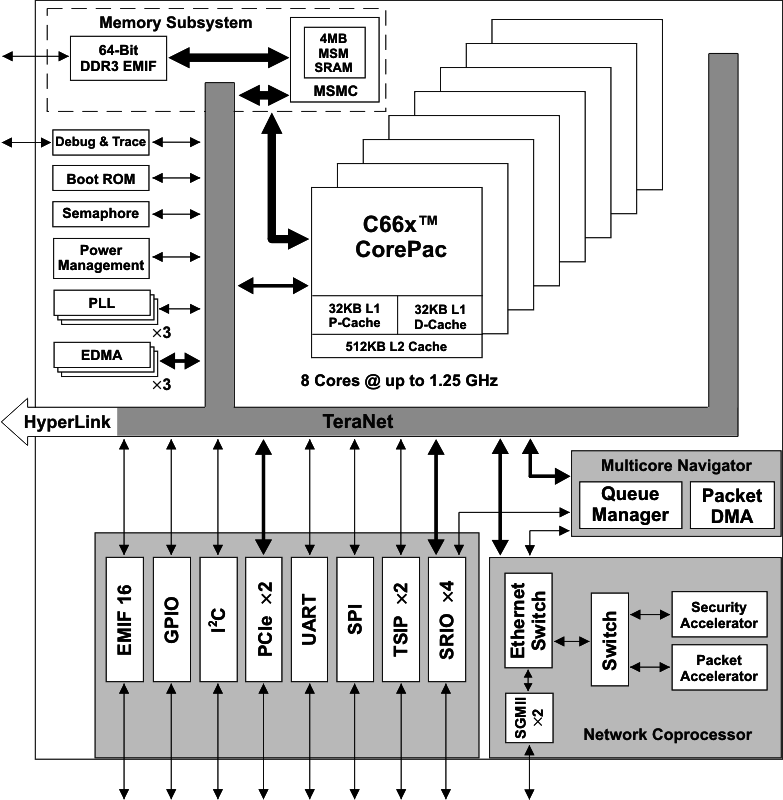
\includegraphics[width=0.99\textwidth]{images/fbd_SPRS691e.png}
        \caption{High-level schematic of the TMS320C6678 architecture. Figure from~\cite{tmsdatasheet}.}
        \label{fig:arch_overview}
    \end{center}
\end{figure}

The TMS320C6678 is based on the Keystone I architecture. The Keystone I architecture specifies a set of hardware elements which enable integration of C66x DSP cores, application specific co-processors and IO \cite{tmsdatasheet}. The Keystone I hardware modules and their connections are presented in the figure \ref{fig:arch_overview}. The points of interest in the figure in the scope of this thesis are the C66x CorePac cores depicted in the middle of the figure, the memory subsystems and its components in the top-left of the figure and the Multicore Navigator depicted in the right edge of the figure.

In the Keystone I architecture there are multiple ways for the C66x cores to communicate with each other, the memory and the peripherals. The methods of communication of specific interest for the experiments in this thesis are communication through shared memory discussed in subsection \ref{subsec:c66memory} and communication through packet based communication manager Multicore Navigator introduced in subsection \ref{subsec:multicorenav}.

The development board used for development of the experiment applications and measurements is an Advantech TMDXEVM6678L. TMDXEVM6678L is an evaluation module for the TMS320C6678 multicore DSP. The evaluation module has 512 megabytes of DDR3 memory which is sufficient for stream processing applications. Another important feature of the evaluation module is the emulator module with USB connectivity. The emulator together with the Code Composer Studio IDE (CCS) make the programming and debugging the experiment programs for the DSPs uncomplicated.~\cite{evmref} CCS version 5.2 is distributed with the hardware evaluation module and was used for development of the experiments in this thesis.

\subsection{C66x DSP}
\label{subsec:c66x}
The hardware platform used in this thesis is the TMS320C6678. The TMS320C6678 consists of eight C66x DSP cores. The C66x is based on the Texas Instruments TMS320C66x instruction set architecture. The TMS320C66x is a very long instruction word architecture, which allows for high amount of instruction level parallelism. The C66x has a total of eight functional units, which operate in parallel. This means that the C66x can dispatch up to eight instructions per cycle. The instructions dispatched in parallel move through pipeline stages simultaneously. Pipelining helps eliminate CPU stalls while waiting for memory operations or other CPU instructions taking multiple cycles complete.~\cite{sprugh7}

Keeping the utilization of the wide pipeline high, the CPU needs to have enough registers to prevent excessive memory access stalling. The CPU has 64 32-bit general purpose registers~\cite{sprugh7}. The C66x is a high-end processor with native support for 32-bit and 64-bit floating point instructions and capability of clock speeds up to 1.4 GHz~\cite{sprugh7}.

\subsection{Memory Hierarchy}
\label{subsec:c66memory}
The TMS320C6678 contains a multi-layer memory hierarchy which can be configured by the user to a large extent. The memory hierarchy in the device consists of L1 and L2 memories for each core, Multicore Shared Memory (MSM) and additionally external memory provided by the evaluation module. In the figure~\ref{fig:arch_overview} the memories are placed inside the subsystems they are part of, MSM can be found in the upper-left corner as part of the memory subsystem.

Each c66x CPU has 32 KB level 1 program cache (L1P), 32 KB level 1 data cache (L1D). Each CPU also has 512 KB of level 2 cache. Both of the L1 caches and the L2 cache can be found in the figure~\ref{fig:arch_overview} as part of the C66x CorePac box. Initially after bootup both L1P and L1D are configured as cache but they can be reconfigured as addressable memory by software. The L2 memory is always configured as addressable memory after reset but can be configured as cache by software. \cite{tmsdatasheet} L2 SRAM addresses are always cached with L1P and L1D whereas external memory addresses are configured noncacheable by default~\cite{cacheguide}.

Configuring the state of the L1 and L2 memories as well as other memory configurations can be handled with software \cite{sprugh7}. CCS automatically handles a lot of the memory mapping needed for applications and provides tools for creating custom configurations.

In PC hardware cache coherence is usually handled automatically by the hardware. In c66x, however, that is not the case. Each c66x core maintains cache coherence between its L1 caches and the L2 cache automatically but programmer needs to manage coherence in most other cases. For example if caching is enabled for an external memory region shared by two cores, explicit cache coherence operations need to be performed before each core can read from or write to the shared region~\cite{cacheguide}.

The evaluation module has 512 MB of DDR3 memory \cite{evmref}. The memory in the evaluation module, as any external memory in other hardware configurations, is accessible through the Multicore Shared Memory Controller (MSMC). The MSMC itself contains 4096KB of shared memory accesible by all cores. In the figure~\ref{fig:arch_overview} the memory subsystem contains the EMIF link to the external memory and the MSMC.

\subsection{Multicore Navigator}
\label{subsec:multicorenav}
The multicore programmability of the TMS320C6678 makes it interesting for this thesis. The device is designed to allow simple co-operation of the DSP cores and provides the required hardware support for that purpose. The core features enabling the multicore programmability are grouped under the name of Multicore Navigator.

Multicore Navigator is the name for a collection of features in Keystone I and II devices, which enables hardware-accelerated, packet-based communication between on-chip devices. Texas Instruments claims the use of specialized hardware for on-chip communication results in significant performance gains when implemented carefully. The design goals stated for the Multicore Navigator in \cite{navigator} are minimizing host interaction and maximizing memory use efficiency.~\cite{navigator}

In Keystone I devices such as the TMS320C6678, the Multicore Navigator provides a hardware queue manager, a special direct memory access for different subsystems called Packet DMA (PKTDMA), and multicore host notifications via interrupts. \cite{navigator} The Texas Instruments OpenEM implementation \ref{chapter:openem} heavily utilizes the features provided by Multicore Navigator.

The Queue Manager on Keystone I architecture devices is a hardware module that manages 8192 queues. Packets are queued and dequeued from the queues by the applications. The Queue Manager is responsible for accelerating the packet communication. In addition to the Queue Manager the Queue Management Subsystem contains two Packed Data Structure Processors (PSDP) which perform tasks related to the queue management and packet communication. For example the PDSP processors can be used to perform accumulation of packets. The accumulation program is given a list of queues to poll. Whenever it finds a descriptor from one of the queues it is watching it will pop the descriptor and place it in a buffer provided by the application. After a pre-determined number of descriptors, or after reaching its time limit, the accumulator program notifies the host processor about the descriptors in the buffer via an interrupt. Use of such firmware offloads the burden of queue polling from the host processors.~\cite{navigator} The TI implementation of OpenEM \ref{chapter:openem} provides its own firmware for the PDSP cores which is utilized by the OpenEM runtime for event scheduling \cite{moerman2014open}.

The PKTDMA is a special DMA utilized by the Multicore Navigator to transfer packet buffers between memory locations. When a packet is sent to a queue The PKTDMA reads the address of the data to be transferred from packet descriptor, transfers the data in one or more data moves and writes the pointer to the data queue specified as the receiver of the packet. The PKTDMA is useful because it allows the program running on a PDSP core to move data in the memory without interrupting the host processors.~\cite{navigator} OpenEM uses PKTDMA to move event buffers to the caches of the core, which is about to receive the event~\cite{moerman2014open}.

\section{PREESM}
\label{sec:preesm}
PREESM is a rapid prototyping framework for multicore development. For understanding the OpenEM framework a way to construct comparable programs with statically scheduled multicore runtime was needed. PREESM provides a way to quickly construct multicore applications for PC as well as for the Texas Instruments multicore DSP used in the experiments. In this chapter the PREESM framework is introduced. First, an overview of the framework is given in subsection \ref{subsec:preesm-overview}. Second, the framework overview, the internal representations used by the framework are described in subsection \ref{subsec:preesm-internal}. Third, scheduling in the PREESM framework is explained in section \ref{sec:preesm-scheduling}. And finally, the memory allocation and code generation in PREESM are explained in section~\ref{sec:preesm-codegen}.

\subsection{PREESM Overview}
\label{subsec:preesm-overview}
PREESM is a collection of tools for rapid prototyping multicore applications. The tools include a graphical editor for the hardware and the software models, code generators for multiple hardware platforms and an automated generator for fixed schedules. The PREESM tools are used through the Eclipse IDE based environment available at~\cite{preesm}.

In PREESM prototypes of applications are constructed by combining hardware and software models with manually created source code and automatically generated schedule. The software model used in PREESM is based on dataflow models of computation and it is discussed in detail in subsection \ref{subsec:preesm-internal}. To create a software model in PREESM the application is divided into actors. The actors contain manually created code, which is often written in side-effect free style to enable parallel execution of the actors, but this is not enforced by the framework. The graphical editor for the software model allows the user to create actors and connect them together using first in first out queues.~\cite{preesm}

The model of the target hardware platform is created using a similar graphical tool as the software model. The hardware model is described in subsection \ref{subsec:preesm-internal}. PREESM parses the graphs of the models and creates a static schedule for the executable. The schedule, the actor implementations and the graphs are inputs for the code generator, which creates the multicore executable.~\cite{pelcat2014preesm} The graphical tools allow the PREESM user to create dependencies between the actors. They also allow a more fine grained control over the code generation by setting estimated actor execution times and selecting the cores on which each actor is allowed to execute.

\begin{figure}[h!]
    \begin{center}
        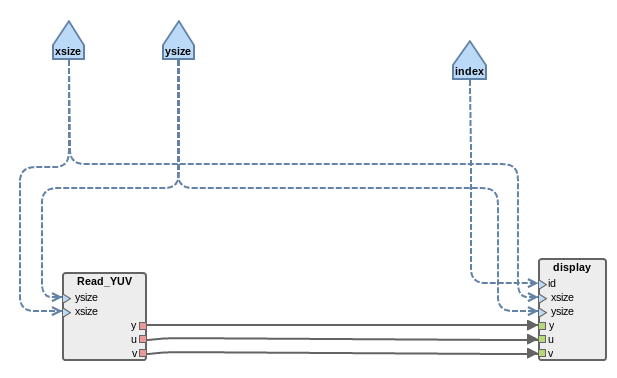
\includegraphics[width=0.99\textwidth]{images/example_preesm_diagram.png}
        \caption{A simple dataflow diagram created with PREESM.}
        \label{fig:preesm_example}
    \end{center}
\end{figure}

\subsection{PREESM Internal Representations}
\label{subsec:preesm-internal}
PREESM applications are created by combining inputs of two different internal representations and manually created source code. The PREESM internal representations are described in this subsection. First, a look is taken at the PREESM algorithm representation PiSDF and second, to the PREESM hardware model.

In PREESM the applications are modeled using a synchronous dataflow based representation of the software called parameterized and interfaced synchronous dataflow model of computation (PiSDF)~\cite{pelcat2014preesm}. PREESM provides graphical tools for editing the dataflow diagram. An example of an dataflow diagram created in PREESM is presented in figure \ref{fig:preesm_example}. The biggest benefit of using synchronous dataflow based model of computation is that deadlock free static schedules can be generated from them~\cite{pelcat2014preesm}. The static schedules generated by PREESM are guaranteed to be deadlock free~\cite{preesm}.

PREESM uses an extended version of SDF called PiSDF \cite{pelcat2014preesm}. PiSDF extends SDF by providing hierarchical graphs based on interfaces and by introducing parameterized actors. An actor in PiSDF can be replaced by a subgraph, which has input and output interfaces. The interfaces insulate the hierarchy levels in terms of schedulability analysis, meaning that schedules can be generated for the subgraphs without knowledge of the higher level models. The parameters are used to configure the production and consumption rates of the actors.~\cite{desnos2013pimm}

An example of a PiSDF graph is presented in figure \ref{fig:preesm_example}. The parameters of the PiSDF model are presented at the top of the figure as pentagons connected to the actors with dashed lines. The actors have input and output ports for parameters and data. The ports define the input and output interfaces of the actors. The actual data paths are the arcs connecting the actors in the bottom of the figure.

The PREESM code generation is aware of the target hardware platform. PREESM uses an internal representation called the System-Level Architecture Model (S-LAM) \cite{pelcat2009system} to describe the target architecture. S-LAM is designed specifically to provide architecture models of high abstraction level for rapid prototyping purposes. S-LAM has good expressive power and it is suitable for modeling heterogeneous architectures as a S-LAM can contain different types of computational resources and communication links.~\cite{pelcat2009system} In the PREESM context however, the typical S-LAM models are simple. For example the S-LAM representing the TMS320C6678 used in experiment \ref{subsec:first-experiment} is quite simple consisting of eight c6678 cores connected through shared memory.

In PREESM the user inputs the speeds of the hardware components of the S-LAM and the speeds of the connections between them. This information is used by the PREESM scheduler to generate a static schedule, that takes communication delays and the component speeds into account, trying to minimize the time spent waiting for communication.~\cite{pelcat2009system}

\subsection{PREESM Scheduling}
\label{sec:preesm-scheduling}
Scheduling multicore applications is not a trivial task, because the execution on a single core is sensitive to what other cores are doing. An unsuccessful schedule may result in the application deadlocking or many other kinds of problems. The approach PREESM takes to overcome the complexity of scheduling multicore applications is using a highly analysable model of computation PiSDF and creating a static schedule based on it. PREESM uses the \textit{List} and \textit{Fast} scheduling methods described in \cite{kwok1997high} for generating a static schedule for multicore platforms. Using these methods PREESM is able to generate a static schedule and guarantee that it is deadlock free.

The reason why multicore applications are created in the first place is the performance increase available through parallelizing the execution. To get a performance increase from parallelizing the application the scheduler must be able to efficiently utilize the multiple cores. The critical measure of performance can be throughput or latency. The designer of the PREESM scheduler has made a decision to focus on so-called latency dominated systems \cite{pelcat2014preesm}. Latency dominated system is defined in \cite{ghamarian2006throughput} as a system where respecting the latency constraint placed upon the system automatically guarantees the satisfaction of the throughput constraint. In other words in the systems PREESM is designed for, each iteration of the application has to fulfill some latency constraint. Fulfilling this latency constraint yields satisfactory throughput. This frees the PREESM scheduler from considering throughput in the scheduling decisions and yields a simpler schedule. Because the scheduler only considers the latency of the execution, the iterations of the algorithm are not interleaved. Instead, all cores are synchronized between the iterations with a barrier.~\cite{pelcat2014preesm}

The execution of the different iterations of the algorithm is not interleaved by the PREESM scheduler. However, intra-iteration interleaving is supported. In intra-iteration interleaving the actors belonging to the same iteration of the algorithm are executed in parallel. \cite{pelcat2014preesm} An example of the intra-iteration interleaving is given in the software pipelining tutorial available at \cite{preesm}.

The dependencies between the actors are defined by the PiSDF model of the application. These dependencies are enough to generate ordering of the actor firings, but to get an efficient schedule the execution times of the actors are needed. The estimated execution times for each actor are provided by the user. The time required for communication between the actors is approximated from the amount out data to be transferred and the speed of the communication links. The data amounts are defined in the actor model and the communication speeds in the S-LAM. With the actor ordering and the timing information, the framework generates a static schedule. \cite{pelcat2014preesm} PREESM framework visualizes the generated schedule with a Gantt chart. An example Gantt chart is presented in figure \ref{fig:preesm_gantt}.

\subsection{PREESM Memory Allocation}
\label{sec:preesm-codegen}
The output of the PREESM framework is a multicore executable. Before the schedule and the user created actors can be combined into an executable, PREESM has to determine how much memory is required for the communication between the actors. The size of every data transfer is determined by the input and output interfaces of the actors and it does not change during the execution. Because the size of the buffers is static, the buffers can be allocated before the execution.~\cite{desnos2012memory}

The data in the communication buffer is considered reserved from the beginning of the execution of the producing actor to the end of execution of the consuming actor. This choice is made to enable custom production rates of the actors. Due to this choice the actors cannot reuse their input buffers as their output buffers. \cite{desnos2012memory} This approach keeps the resulting executable simple but it results in extra copying of buffers between the actors.

In the simple case where the producing and the consuming actors execute on the same core and are not dependent on any other actors, simple copying of buffers is enough. However when the producing actor executes on a different core than the consuming actor, the cores need to synchronize before the consuming actor can start to execute. If the user provided estimates for the execution times of the actors are accurate, the synchronizations should not cause a lot of waiting.~\cite{pelcat2014preesm}

With the memory allocations computed, the framework can create an executable. The structure of the complete application follows the template provided by the framework. The memory allocations are handled in the initialization. After the initialization the cores enter loops where the static schedule for each core is laid out as interleaved calls to actor implementations, memory operations to move the data between the buffers and synchronization barriers.

\section{Video Streams}
\label{sec:video-streams}
Many different video stream formats are needed to capture, transfer and store videos. Raw video material requires a lot of space to store and a lot of bandwidth to transfer but when the video data is edited, the part of the video stream that is being edited has to be in unpacked format. In this section two standards related to video streams are explained. First the YUV color specification and second the CIF frame resolution format.

\subsection{YUV Format}
\label{subsec:yuv}
YUV color space is used in encoding colors of images and videos. The YUV color system is used for example in encoding the colors of television broadcasts using the PAL or NTSC systems. The YUV color space is designed with the human perception in mind, meaning the channels are selected so that compression artifacts and other errors are more likely masked by human perception. This allows for reduced bandwith compared to RGB encoded colors. The Y channel corresponds to the luminance of the image. Luminance means the perceived brightness. In a black and white image or video only the Y channel is used. The U and V channels are called the chrominance channels and they encode the color component of the image.~\cite{jack2011video}

In digital media YUV term is commonly used to refer to YCbCr, which is a way of encoding RGB color information. Y' (Y prime) is called luma and is distinct from the Y channel of the analog YUV system. The luma channel is a non-linear encoding of the light intensity. Cb and Cr are the blue-difference and red-difference components respectively. It is common to store the luma channel at a higher resolution than the chroma channels to save bandwidth. This process is called chroma sub-sampling. Humans are more sensitive to the brightness of the image than the color of the image and thus the lower resolution of the chroma channels causes less noticeable artifacts.~\cite{jack2011video}

\subsection{Common Intermediate Format}
\label{subsec:cif}
Common Intermediate Format or CIF is a standardization of the horizontal and vertical resolutions of pixels in video signals. The CIF pixels are non-square with an aspect ratio of approximately 1.222:1. The standard defines multiple resolutions such as the CIF 352x288 and QCIF for quarter CIF 176x144.CIF resolutions were designed to be easily convertible to the PAL and NTSC systems.~\cite{telecommunication1993itu}

\section{Canny edge detector}
\label{sec:canny}
Edge detection is an important tool in image processing and computer vision. Many image processing and computer vision algorithms operate on detected edges. The quality of the detected edges is important for the algorithms using them as input. In his 1986 paper John F. Canny \cite{canny1986computational} lays out the mathematical criteria for successful edge detection and presents an algorithm, which achieves decent edge detection performance. The algorithm is suitable for implementation on DSPs. The Canny edge detection algorithm consists of five steps presented in the following list.

\begin{enumerate}
    \item{Noise reduction}
    \item{Finding the intensity gradient of the image}
    \item{Non-maximum suppression}
    \item{Double thresholding}
    \item{Edge tracking by hysteresis}
\end{enumerate}

In the canny edge detector the image is first filtered with a gaussian filter to reduce the amount of noise in the image. Second, the changes in the intensity in the image are detected using an image gradient operator such as the sobel operator. The third step improves the accuracy of the edge detection by suppressing all but the strongest responses to the detected edges, in practice ``thinning'' the edges. The fourth step classifies the edge pixels to three classes separated by empirically determined threshold values. The pixels with gradient value above the high threshold are marked strong pixels and the pixels with gradient value below the low threshold are suppressed. In the fifth step the remaining weak pixels with gradient values below the high threshold are preserved or suppressed according to the presence of strong pixels in their neighborhood. Detailed description of the algorithm is presented in the original paper by Canny \cite{canny1986computational}, information about implementing a canny edge detector is available in \cite{gonzalez2008digital} and comparison of its performance to other edge detectors can be found in \cite{maini2009study}.

In this section the phases of canny edge detector are described in the order they are used in Canny filter. First, the gaussian filter is introduced in subsection \ref{subsec:gauss}. The sobel filter is looked at next in subsection \ref{subsec:sobel}. After the sobel filter, the edge responses are pruned in three phases. The three phases are presented in subsection \ref{subsec:canny-edge-pruning}.

\subsection{Gaussian filter}
\label{subsec:gauss}
Gaussian filtering is used for multiple purposes in digital image processing. In the canny edge detector the gaussian filter is used to reduce noise in the processed images. The gaussian filter works by convolving a gaussian function with the input signal. Gaussian function is non-zero everywhere which means it would theoretically require an infinite convolution window. Since the function decays rapidly it is often reasonable to truncate the function and use small windows.~\cite{gonzalez2008digital} 

Calculating the convolution with a truncated function means in practice that every pixel in the filtered image has an intensity value computed by taking a weighted average of the neighboring pixels in the input image. The weights are pre-calculated from the gaussian function, giving the highest weight to the pixel in the center of the window. The gaussian filter displayed in figure \ref{fig:gaussmat} was calculated with $\sigma$ = 1.3. The filtered image has a smoothed appearance compared to the original image.

\begin{figure}
    \begin{displaymath}
        B = \frac{1}{159}\begin{bmatrix}
             2 & 4 & 5 & 4 & 2 \\
             4 & 9 & 12 & 9 & 4 \\
             5 & 12 & 15 & 12 & 5 \\
             4 & 9 & 12 & 9 & 4 \\
             2 & 4 & 5 & 4 & 2 \\
        \end{bmatrix} \ast A
    \end{displaymath}
    \caption{Convolution with a gaussian kernel computed with $\sigma = 1.3$. The convolution operation is denoted by the asterisk.}
    \label{fig:gaussmat}
\end{figure}

\subsection{Sobel filter}
\label{subsec:sobel}
The actual edge detection in the canny edge detector begins with determining the changes in the intensity of the image. This is done by applying the sobel operator to the input image. The sobel operator is a discrete differentiation operator. It consists of two 3x3 kernels which are convolved with the image to approximate the derivatives. The two kernels represent horizontal and vertical changes. At each point in the image the resulting gradient approximations are combined giving an approximate gradient magnitude. \cite{gonzalez2008digital} The convolution operations are presented in figure \ref{fig:sobelmat}.

\begin{figure}
    \begin{displaymath}
        G_{x} = \begin{bmatrix}
            -1 & 0 & +1 \\
            -2 & 0 & +2 \\
            -1 & 0 & +1 \\
        \end{bmatrix} \ast A
    \end{displaymath}
    \begin{displaymath}
        G_{y} = \begin{bmatrix}
            -1 & -2 & -1 \\
            0 & 0 & 0 \\
            +1 & +2 & +1 \\
        \end{bmatrix} \ast A
    \end{displaymath}
    \caption{The 3x3 Sobel kernels used in the application to compute the gradient approximation. $G_{x}$ is the horizontal gradient approximation at given pixel and $G_{y}$ is the vertical gradient approximation. The asterisk denotes the convolution operation.}
    \label{fig:sobelmat}
\end{figure}

\subsection{Canny Edge Pruning}
\label{subsec:canny-edge-pruning}
Canny edge detector is designed to detect edges accurately and as unambiguously as possible. To make unambiguous detections, each edge in the input image should produce only one edge response. For this purpose Canny edge detector employs \textbf{non-maximum suppression}. Non-maximum suppression works on the gradient image that was calculated in the previous phase. For each pixel in the gradient images, non-maximum suppression compares the gradient value to the adjacent pixels in positive and negative gradient directions. The pixel is preserved only if it has the largest gradient value compared to its neighbors.~\cite{gonzalez2008digital}

The non-maximum suppression outputs an image where the edge responses have been pruned to single response per edge, but there still remain gradient pixels that correspond to noise or other uninteresting variations in the image. The detection quality is further improved by applying two thresholds to the output of the non-maximum suppression phase. In the literature this phase is called \textbf{double thresholding}. If the gradient value of a pixel is higher than the high threshold, the pixel is marked as a strong pixel. If the value is lower than the high threshold but higher than the low threshold, the pixel is marked as weak pixel. Pixels with gradient values lower than the low threshold are automatically discarded. The threshold values are determined empirically.~\cite{gonzalez2008digital}

In the final phase of the Canny edge detector, called \textbf{edge tracking by hysteresis} the strong pixels are used to determine which of the weak pixels to keep and which to discard. A weak pixel is preserved if there is at least one strong pixel among its eight neighboring pixels. If there are no strong pixels in the neighborhood the weak pixel is discarded.~\cite{gonzalez2008digital}
